\documentclass[../book.tex]{subfiles}

\chapter{Machines finding functions}
\label{ch:function}

\begin{quote}
Because of a gradient that no doubt characterizes our cultures,
discursive formations are constantly becoming epistemologized
\autocite[195]{Foucault_1972}
\index{Foucault, Michel!on epistemologization}
\end{quote}

`All knowledge,' hypothesises Pedro Domingos, `past, present,and future
can be derived from data by a single, universal learning algorithm'
\autocite[25]{Domingos_2015a}. \index{Domingos, Pedro!on algorithms}
\index{algorithm!variety of} How will the `single, universal' algorithm
learn, how will it `epistemologize,' to use Foucault's term, `our
cultures'?

In practice, the opening pages of machine learning textbooks often warn
or enthuse about the profusion of techniques, algorithms, tools and
machines. \index{machine learners!variety of|(} `The first problem
facing you', cautions Domingos readers of the \emph{Communications of
the ACM}, `is the bewildering variety of learning algorithms available.
Which one to use? There are literally thousands available, and hundreds
more are published each year \autocite[1]{Domingos_2012}.
\index{Domingos, Pedro!on algorithms in machine learning} 'The
literature on machine learning is vast, as is the overlap with the
relevant areas of statistics and engineering' echoes David Barber in
\emph{Bayesian Reasoning and Machine Learning}\autocite[4]{Barber_2011};
`statistical learning refers to a vast set of tools for understanding
data' writes James and co-authors in an \emph{Introduction to
Statistical Learning with R} \autocite[1]{James_2013}; or writing in in
\emph{Statistical Learning for Biomedical Data} the biostatisticians
James Malley, Karen Malley and Sinisa Pajevic `freely admit that many
machines studied in this text are somewhat mysterious, though powerful
engines' \autocite[257]{Malley_2011}. In \emph{Thoughtful Machine
Learning} Matthew Kirk exacerbates the situation: `flexibility is also
what makes machine learning daunting. It can solve many problems, but
how do we know whether we're solving the right problem, or actually
solving it in the first place?' \autocite[ix]{Kirk_2014}.
\index{Kirk, Matthew} The prefatory comments from Domingos, Barber,
James, Malley and Kirk suggest a rampant even weed-like abundance of
machine learners, as does the 700 or so pages of \emph{Elements of
Statistical Learning}. Much learning of machine learning work, at least
for machine learners, concerns not so much implementation of particular
techniques (neural network, decision tree, support vector machine,
logistic regression, etc.), but rather navigating the maze of methods
and variations that might be relevant to a particular situation.
\index{learning!machine learning} How does this dual effect of profuse
accumulation and the ideal a single, universal machine learner arise and
hold together?

\begin{figure}
  \centering
      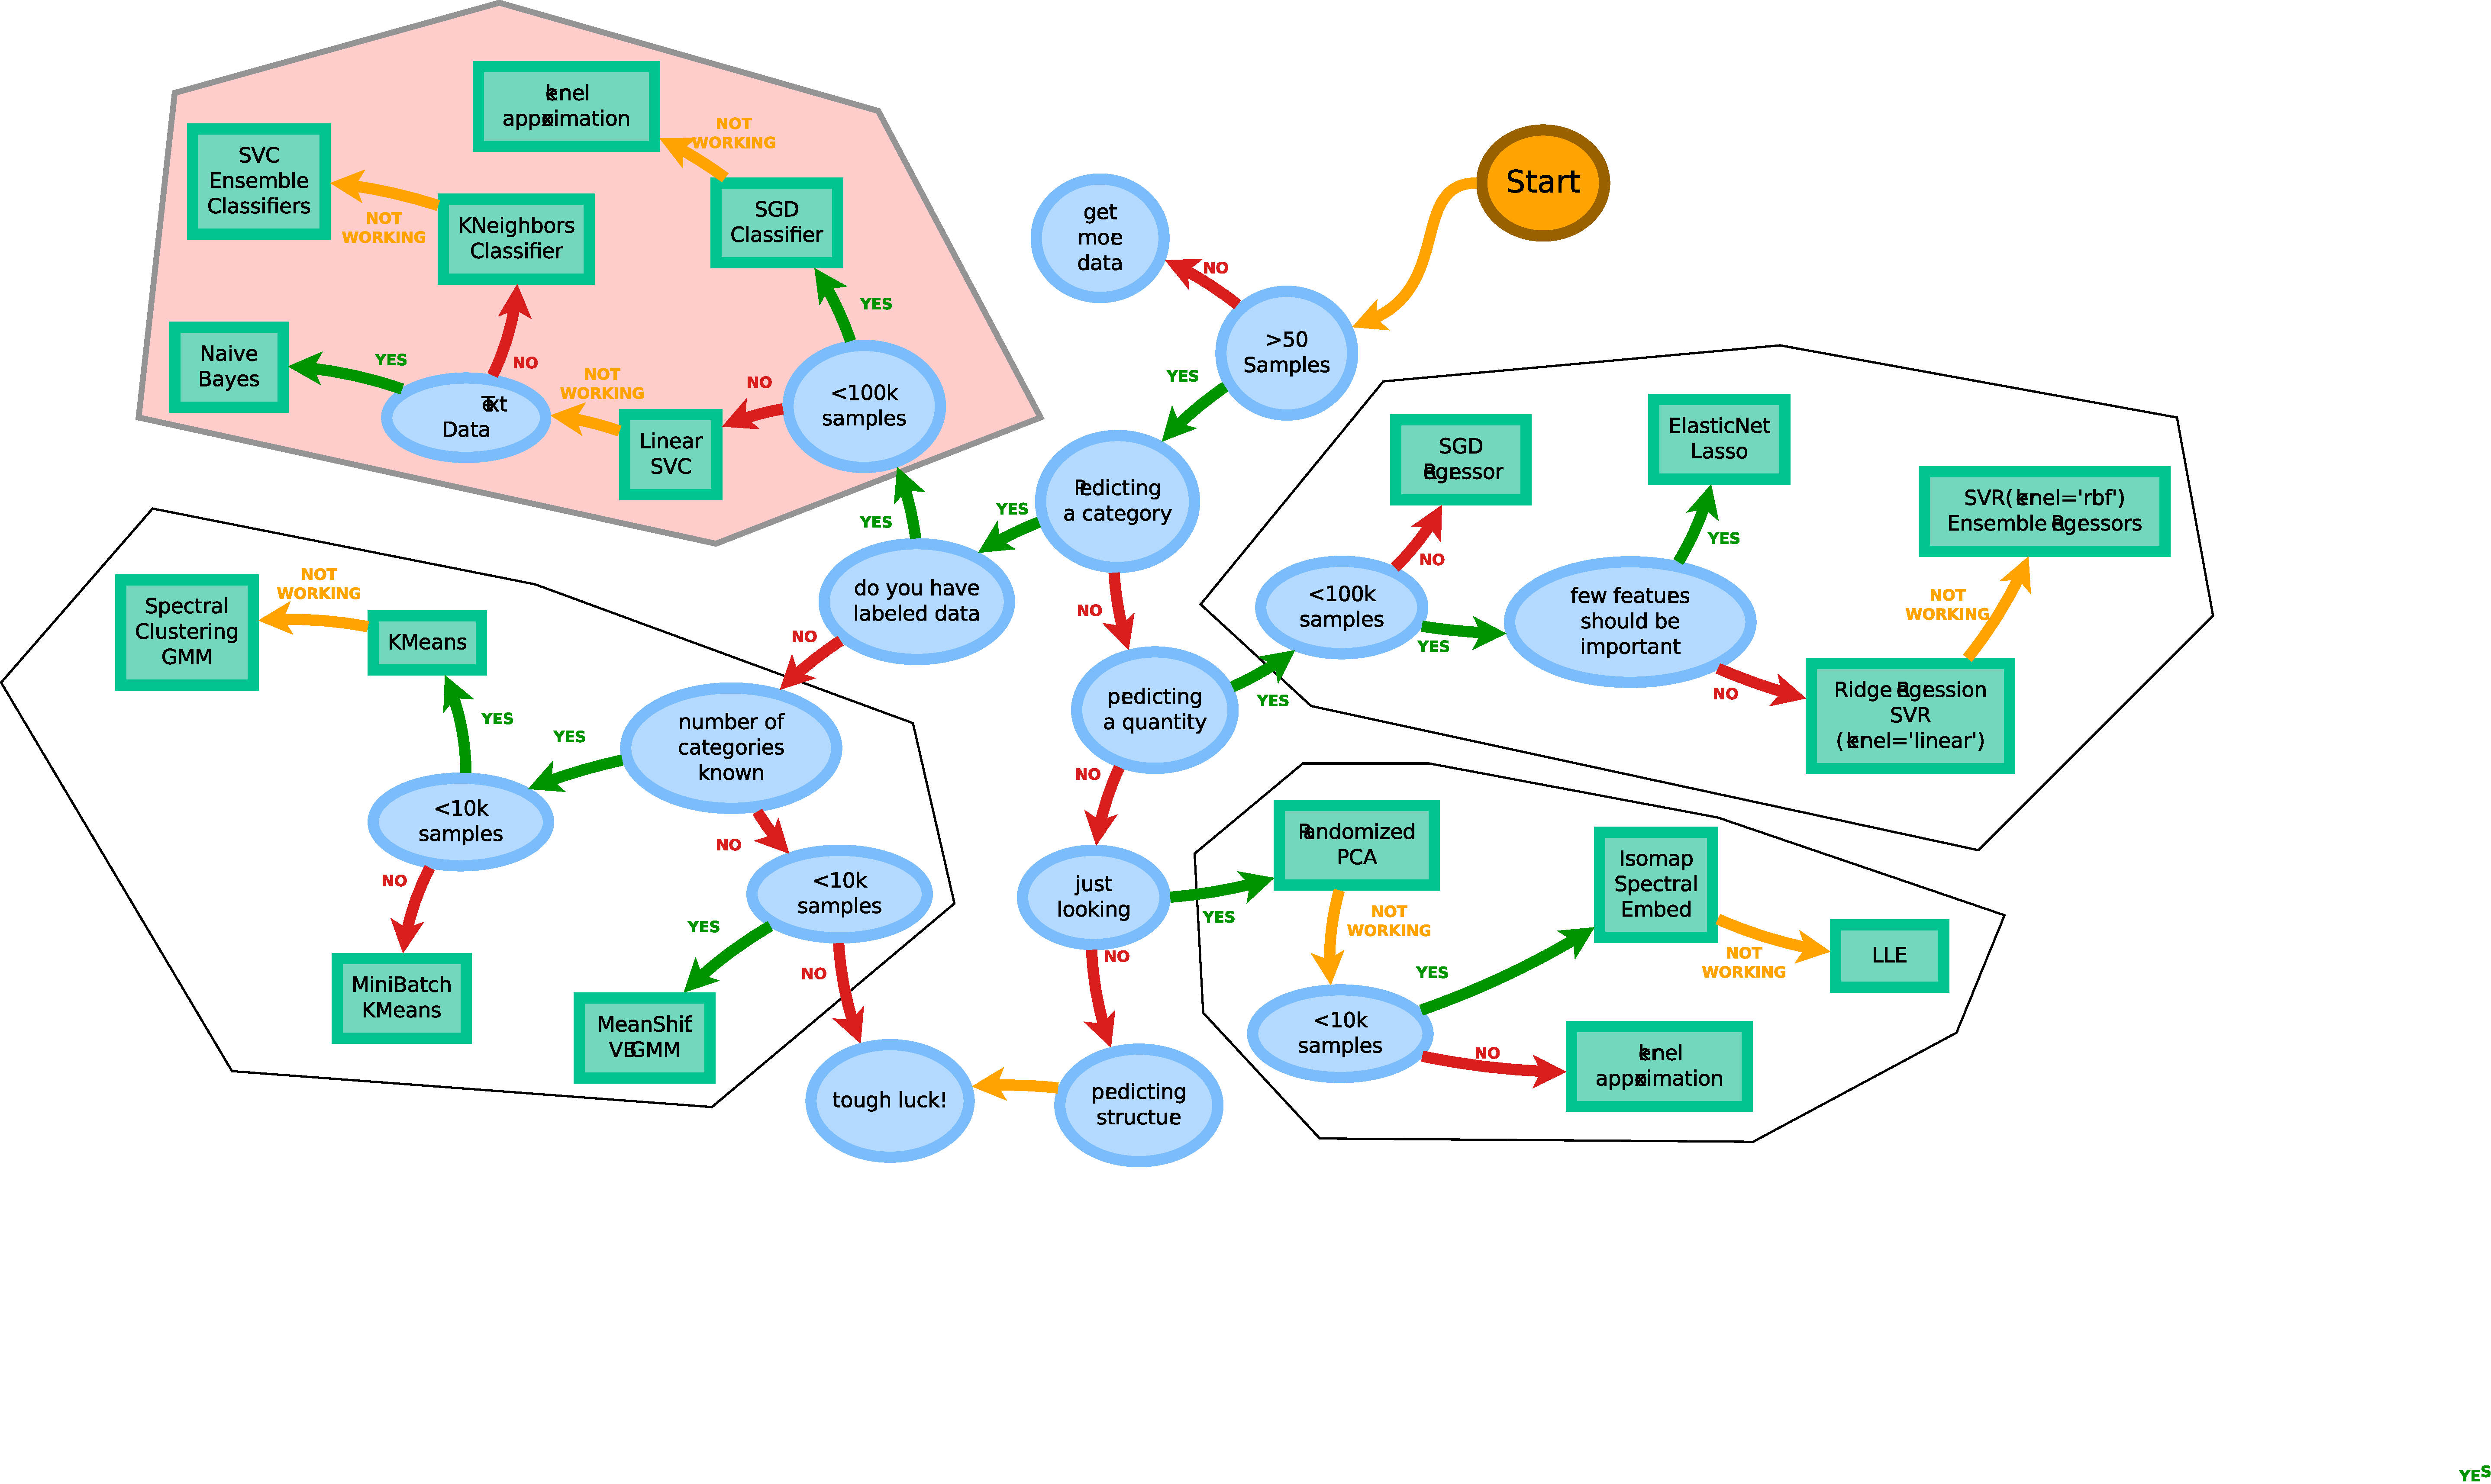
\includegraphics[width=0.95\textwidth]{figure/ml_map_scikit.pdf}
        \caption[\textt{scikit-learn} map of machine learners]{\texttt{scikit-learn} map of machine learning techniques }
  \label{fig:mapping_functions}
\end{figure}

\index{Python!packages!\texttt{scikit-learn}}

The machine learners I have just cited present that profusion as a
problem of the piling up of techniques. As the authors of textbooks and
how-to-manuals, they attempt to manage it by providing, indexes, maps
and guides to the bewildering variety of machine learners.
\emph{Elements of Statistical Learning} deploys tables, overviews,
theories of statistical modelling, model assessment and comparison
techniques to aid in navigating them.

Parallel and complementary mappings accompany software libraries. The
visual map of machine learning techniques shown in Figure
\ref{fig:mapping_functions} comes from a machine learning library
written in \texttt{Python,} \texttt{scikit-learn}
\autocite{Pedregosa_2011}. \index{Python!library!\texttt{scikit-learn}}
This software library is widely used in industry, research and commerce.
In contrast to the pedagogical expositions, theoretical accounts or
guides to reference implementation, or the many overlapping packages in
\texttt{R}, code libraries such as \texttt{scikit-learn} order the range
of techniques by offering recipes and maps for the use of the
\emph{functions} the libraries supply. \index{function} The branches in
the figure lay down paths through the profusion of techniques as a
decision tree.\footnote{Similarly, for \texttt{R} code, the
  \emph{Comprehensive R Archive Network} tabulates key libraries of
  \texttt{R} code in a machine learning `task view'
  \autocite{Hothorn_2014}. \index{R!task views of}}
\index{machine learners!variety of|)}
\index{programming languages!R!Comprehensive R Archive Network}

The architecture of software libraries itself classifies and orders
machine learners. \texttt{Scikit-learn} for instance comprises a number
of sub-packages. Modules such as \texttt{lda} (linear discriminant
analysis), \texttt{svm} (support vector machine) or \texttt{neighbors}
(\emph{k} nearest neighbours) point to well-known machine learners,
whilst \texttt{cross-validation} or \texttt{feature\_selection} refer to
ways of testing models or transforming data respectively. These
divisions, maps and classifications help order the techniques, but they
obscure the process that first generates a competing profusion of
machine learners.

If, as I have suggested earlier, we understand knowledge in terms of the
radically re-conceptualised statements that Foucault described in
\emph{The Archaeology of Knowledge}, then statements comprise various
units (sentences, series, tables, propositions, diagrams, equations,
numbers) mapped to a field of objects, subject positions and domains of
coordinations and reuse by an enunciative function
\autocite[106]{Foucault_1972}. Confronted by a profusion of machine
learners and the idea of a single, universal machine learning, an
archaeological analysis attends to the enunciative function that
multiplies meanings and
operations.\index{archaeology!profusion of elements}

We might understand the enunciative function
\index{enunciative function} as the generative process that proliferates
machine learners. The listing and mapping of accumulated techniques,
whether in the form of textbooks such as \emph{Elements of Statistical
Learning} or a code library such as \texttt{scikit-learn}, together with
the many attempts to unify them (Domingo's `single, universal
algorithm', \texttt{scikit-learn}`s map, \emph{Elements of Statistical
Learning}'s statistical theory) suggests a commonality in the production
of statements. As I will argue in this chapter, there are so many
techniques, algorithms and ways of deriving knowledge from data in
machine learning because statements are actually rare in this
operational formation. 'Because statements are rare,' writes Foucault,
`they are collected in unifying totalities, and the meanings to be found
in them are multiplied' \autocite[120]{Foucault_1972}.
\index{statements!rarity of}

\section{Learning functions}\label{learning-functions}

\begin{table}[ht]
\centering
\begingroup\tiny
\begin{tabular}{p{0.1\textwidth}p{0.5\textwidth}p{0.3\textwidth}p{0.10\textwidth}}
  \hline
Year & Title & Keywords & Citations \\ 
  \hline
1992 & Comparison Of 3 Different Methods For Automated Classification Of Cervical Cells & machine classification; cervical cells; automated prescreening; discriminant function analysis; decision tree classification; neural network &  29 \\ 
  1994 & Minimization Methods For Training Feedforward Neural Networks & feedforward neural network training; numerical optimization techniques; neural function approximation; error back propagation; conjugate gradient; quasi-newton &  76 \\ 
  1995 & Recurrent Radial Basis Function Networks For Adaptive Noise Cancellation & radial basis function network; noise cancellation; nonlinear filtering &  65 \\ 
  1997 & Comparing Support Vector Machines With Gaussian Kernels To Radial Basis Function Classifiers & clustering; pattern recognition; prototypes; radial basis function networks; support vector machines & 405 \\ 
  1998 & Rbf Nets, Mixture Experts, And Bayesian Ying Yang Learning & radial basis function network; mixture of experts; bayesian ying-yang learning; model selection; coordinated competitive learning; fast computation; adaptive algorithm; financial time series; curve fitting &  65 \\ 
  2001 & Greedy Function Approximation: A Gradient Boosting Machine & function estimation; boosting; decision trees; robust nonparametric regression & 900 \\ 
  2002 & Technical Update: Least Squares Temporal Difference Learning & reinforcement learning; temporal difference learning; value function approximation; linear least-squares methods &  50 \\ 
  2004 & An Interactive Approach For Cbir Using A Network Of Radial Basis Functions & content-based image retrieval; digital library; relevance feedback; machine learning; radial basis function network; nonlinear human perception &  41 \\ 
  2005 & Bankruptcy Prediction Using Support Vector Machine With Optimal Choice Of Kernel Function Parameters & bankruptcy prediction; support vector machine; grid-search; kernel function; back-propagation neural networks & 133 \\ 
  2005 & Partially Supervised Classification Of Remote Sensing Images Through Svm Based Probability Density Estimation & probability density function (pdf) estimation; supervised classification; support vector machines (svms); unknown classes &  39 \\ 
  2006 & Recent Progresses In The Application Of Machine Learning Approach For Predicting Protein Functional Class Independent Of Sequence Similarity & machine learning method; neural network; protein function prediction; protein sequence; support vector machine &  38 \\ 
  2006 & Improving Rbf Networks Performance In Regression Tasks By Means Of A Supervised Fuzzy Clustering & fuzzy clustering; fuzzy c-means; radial basis function neural networks; linear regression models &  37 \\ 
  2006 & An Explicit Description Of The Reproducing Kernel Hilbert Spaces Of Gaussian Rbf Kernels & gaussian radial basis function (rbf) kernel; reproducing kernel hilbert space; support vector machine &  28 \\ 
  2006 & The Effect Of Different Basis Functions On A Radial Basis Function Network For Time Series Prediction: A Comparative Study & radial basis function network; basis function; basis width &  72 \\ 
  2006 & Predicting Rrna , Rna , And Dna Binding Proteins From Primary Structure With Support Vector Machines & rrna-binding protein; rna-binding protein; dna-binding protein; protein function prediction; support vector machines (svms) &  49 \\ 
  2006 & Structural Bioinformatics Prediction Of Membrane Binding Proteins & protein-membrane interactions; function annotation; support vector machines; peripheral proteins; protein function prediction &  29 \\ 
  2009 & Time Series Prediction Using Rbf Neural Networks With A Nonlinear Time Varying Evolution Pso Algorithm & time series prediction; radial basis function networks; particle swarm optimization; nonlinear time-varying evolution &  49 \\ 
  2009 & Dictionary Learning For Sparse Approximations With The Majorization Method & block relaxation methods; constrained optimization; dictionary learning; majorization methods; sparse approximation; surrogate function optimization method &  27 \\ 
  2009 & Computational Chemistry Study Of 3d Structure Function Relationships For Enzymes Based On Markov Models For Protein Electrostatic, Hint, And Van Der Waals Potentials & 3d-qsar; markov chains; protein structure-function relationship; electrostatic potential; van der waals potential; hint potential; enzymes; machine learning; artificial neural networks &  33 \\ 
  2011 & Forecasting Stock Indices Using Radial Basis Function Neural Networks Optimized By Artificial Fish Swarm Algorithm & artificial fish swarm algorithm; radial basis function neural network; k-means clustering algorithm; data mining; shanghai stock exchange index &  66 \\ 
   \hline
\end{tabular}
\endgroup
\caption{Sample of highly cited machine learning publications referring to "function" in title or keyword} 
\label{tab:function_in_ml}
\end{table}

The rarity of statements amidst the profusion of machine learners
revolve around a single operator, the \gls{function}.\footnote{I discuss
  the sense of function as operation or process in chapter
  \ref{ch:genome}. There I suggest that this important sense of function
  as operation or process, a sense that has underpinned transformations
  in life, social and clinical sciences may be shifting towards a
  different ordering. \index{function!transformation in meaning of}}
Table \ref{tab:function_in_ml} shows the titles and author-supplied
keywords of a sample of well-cited machine learning publications. In
these randomly chosen publications, mathematical functions -- `kernel
function,' `discriminant function,' `radial basis function' -- mingle
with biological and engineering functions -- `protein-binding function,'
`intestinal motor function', or `rules to control locomotion.'
Mathematical functions, however, dominate. Machine learners `find',
`estimate,' `approximate,' `analyse' and sometimes `decompose'
mathematical functions. The primary mathematical sense of a function
refers to a relation -- a mapping -- between sets of values or
variables. (A variable is a symbol that can stand for a set of numbers
or other values.) A function is one-to-one relation between two sets of
values. It maps a set of arguments (inputs) to a set of values (outputs,
or to use slightly more technical language, it maps between a
\emph{domain} and a \emph{co-domain}.) As we have already seen,
mathematical functions are often written in formulae of varying degrees
of complexity. They are of various genres, provenances, textures and
shapes: polynomial functions, trigonometric functions, exponential
functions, differential equations, series functions, algebraic or
topological functions, etc. Various fields of mathematics have pursued
the invention of functions. In machine learning and information
retrieval, important functions include the logistic function (discussed
below), probability density functions (PDF) for different probability
distributions (Gaussian, Bernoulli, Binomial, Beta, Gamma, etc. See
chapter \ref{ch:probability}), \index{probability!distribution}
\index{function!mathematical} and error, cost, loss or objective
functions (these four are almost synonymous).
\index{cost function|see{function!cost}} (The latter group I discuss
below because they underpin many claims that machine learners learn.)
\index{function!variety of}

As we will see, from the perspective of the function, machine learning
can be understood as a function-finding operation.
\index{machine learning!as function-finding} Implicitly or explicitly,
machine learners find a mathematical expression -- a function --
approximating the social, technical, financial, transactional,
biological, brain, heart or group process that flowed the data in
question into vector space\index{vector space!data in}. Regardless of
the application, no single mathematical function perfectly or uniques
expresses data. Many if not infinite functions can approximate any given
data. Even if there was a master algorithm, therefore, it would be
concerned with a field of functions, and it would entail observation,
classification and selection (finding, in short) in deriving knowledge
from data. \index{function!variations of}

\section{Supervised, unsupervised, reinforcement learning and
functions}\label{supervised-unsupervised-reinforcement-learning-and-functions}

The capacity of machine learners to learn is very closely linked to
forms of observation that co-produce knowledge. The optics of this
observation of machine learners vary but they are always partial or
incomplete, partly because of the dimensionality of vector space and
partly because of the domains in which machine learning operates. While
the field is pragmatic in its commitment to classification and
prediction (although in certain ways, curiously idealistic too in its
constant reuse of well-worked datasets such as \texttt{iris} or
\texttt{South\ African\ heart\ disease}), it distinguishes between three
broadly different kinds of \emph{learning} -- supervised, unsupervised,
and reinforcement -- in terms of their observability.
\index{machine learning!learning|(} \emph{Elements of Statistical
Learning} presents the distinction between supervised and unsupervised
learning:

\begin{quote}
With supervised learning there is a clear measure of success or lack
thereof, that can be used to judge adequacy in particular situations and
to compare the effectiveness of different methods over various
situations. Lack of success is directly measured by expected loss over
the joint distribution \(Pr(X,Y)\). This can be estimated in a variety
of ways including cross-validation. In the context of unsupervised
learning, there is no such direct measure of success. \ldots{} This
uncomfortable situation has led to heavy proliferation of proposed
methods, since effectiveness is a matter of opinion and cannot be
verified directly. \autocite[486-7]{Hastie_2009}
\end{quote}

Supervised learning in general terms constructs a model by training it
on some sample data (the training data \index{data!training} ), and then
evaluating the model's effectiveness in classifying or predicting unseen
test data \index{data!test} whose actual values are already known. The
`clear measure of success' in relation to in so-called `supervised
learning' is of relatively recent date.\footnote{Only in the mid-1980s
  were the first theories of algorithmic learning formalised
  \autocite{Valiant_1984}.} \index{machine learning!supervised}
Unsupervised machine learning techniques generally look for patterns in
the data without any training or testing phases (for instance,
\emph{k}-means or principal component analysis do this, and both
techniques have been heavily used for more than fifty years). In both
supervised and unsupervised learning, machine learners observe how a
function (or functions) changes as a model transforms, partitions or
maps the data. \index{machine learner!\textit{k}-means}
\index{machine learner!principal component analysis}

Viewed as enunciative function, machine learning makes statements
through operations that treat functions as \glspl{partial observer}.
\index{function!as partial observer} At the same time, opacity -- `no
direct measure of success' -- is generative in machine learning.
\index{partial observer|see{function!as partial observer}}
\emph{Elements of Statistical Learning} admits that success cannot be
measured and that this inaccessible difficulty has led to proliferating
methods, transformations and changes. If, as the first part of the
quoted text puts it, supervised learning has a clear `measure of
success,' that success only seems to encourage further variations and
comparisons that end up proliferating machine learners, their
publications and their software implementations.
\index{machine learning!learning|)}

\section{Which function operates?}\label{which-function-operates}

\index{function!mathematical|(} Differences between machine learners can
be described using mathematical functions. That is, machine learners
operate as functions and observations of those operations also
constitute functions. Functions instantiate \emph{both} the operations
and the ordering of those operations.

For instance, classifiers, or machine learners that classify, are often
identified directly with functions:

\begin{quote}
A classifier \ldots{} is a function \(d(\mathbf{x})\) defined on
\(\mathcal{X}\) so that for every \(\mathbf{x}\), \(d(\mathbf{x})\) is
equal to one of the numbers \(1, 2, ..., J\) \autocite[4]{Breiman_1984}
\index{Breiman, Leo!on classifiers} \index{function!as classifier}
\end{quote}

Writing in the 1980s, the statistician Leo Breiman identifies
classifiers -- perhaps the key operational achievement of machine
learning and certainly the catalyst of many applications -- with
functions. A classifier \emph{is} a function \(d(\mathbf{x})\) where is
\(\mathbf{x}\) is the data and \(d\) ranges over numbers that map onto
categories, rankings or or other forms of order and belonging (for
instance, \texttt{cat} or \texttt{not\ cat} in the case of
\texttt{kittydar}).

The identification of machine learning with functions appears in the
first pages of most machine learning textbooks. Viewed operationally,
learning in machine learning means finding a function that can identify
or predict patterns in the data. As \emph{Elements of Statistical
Learning} formulates it,

\begin{quote}
our goal is to find a useful approximation \(\hat{f}(x)\) to the
function \(f(x)\) that underlies the predictive relationship between
input and output \autocite[28]{Hastie_2009}.
\index{function!as approximation}
\end{quote}

This statement of learning compresses several layers in the function. It
posits the existence of \emph{the} function that generated the data as a
foundation. This function figures as a ground truth existentially
imputed to the world. It also refers to `finding \ldots{}
\(\hat{f}(x)\)', where the'\^{}`indicates a 'useful' approximation. A
leading theorist of learning theory Vladimir Vapnik echoes the statement
of learning as a function: `learning is a problem of \emph{function
estimation} on the basis of empirical data'
\autocite[291]{Vapnik_1999}.\footnote{Vapnik is said to have invented
  the support vector machine, one of the most heavily used machine
  learning technique of recent years on the basis of his theory of
  computational learning. Chapter \ref{ch:pattern} discusses the support
  vector machine.} \index{Vapnik, Vladimir!on learning} The use of the
term `learning' in machine learning displays affiliations to the field
of artificial intelligence, but the `function-fitting paradigm' as
\autocite[29]{Hastie_2009} terms it, emphasises this double layering of
function as an observed approximation. Most importantly, \emph{learning}
here is understood as finding. Despite many differences in the framing
of the techniques, all accounts of machine learning, even those such as
\emph{Machine Learning for Hackers} \autocite{Conway_2012} that eschew
any explicit recourse to mathematical formula, rely on the formalism and
modes of thought associated with mathematical functions. Whether they
are seen as forms of artificial intelligence or statistical models, the
formalisms are directed to build `a good and useful approximation to the
desired output' \autocite[41]{Alpaydin_2010}, or, put more
statistically, `to use the sample to find the function from the set of
admissable functions that minimizes the probability of error'
\autocite[31]{Vapnik_1999}. \index{function!mathematical|)}

The superimposed or doubling of function as operation and observer is
hardly ever explicitly mentioned by machine learners.
\index{function!as operation and observer} The pages of
\autocite{Hastie_2009} present a series of `functions': quadratic
function, likelihood function, sigmoid function, loss function,
regression function, basis function, activation function, penalty
functions, additive functions, kernel functions,step function, error
function, constraint function, discriminant function, probability
density function, weight function, coordinate function, neighborhood
function, and the list goes on. This mixed list draws from a pool of
several hundred mathematical functions commonly used in science and
engineering.\footnote{The U.S. National Institute of Standards published
  \emph{The Handbook of Mathematical Functions} in 1965
  \autocite{Abramowitz_1965}. This heavily cited volume, now also
  \href{http://dlmf.nist.gov}{versioned online} lists hundreds of
  functions organised in various categories ranging from algebra to zeta
  functions. While a number of the functions and operations catalogued
  there surface in machine learning, machine learners implement, as we
  will see, quite a narrow range of functions.} Clearly neither machine
learners or critical researchers can expect to understand the
functioning of all these functions in any great detail. While this
prickly list of terms begins confirms the salience of functions in
machine learning (as perhaps in many other science and engineering
disciplines), certain basic difference between functions might be a way
to map the interplay of operational and observational functions. We can
already see in this list that function are diverse. Sometimes, the
function refers to a mathematical form -- `quadratic,' `coordinate',
`basis' or `kernel'; sometimes it refers to statistical considerations
-- `likelihood', `regression', `error,' or `probability density'; and
sometimes it refers to some other concern that might relate to a
particular modelling device or diagram -- `activation,' `weight',
`loss,' `constraint,' or `discriminant.'

\section{What does a function learn?}\label{what-does-a-function-learn}

We wish to know: in what sense does a machine learner learn? This
question can now be re-framed: how do machine learners find functions?
For critical thought, this is a vexing question, for if function-finding
agency inheres in machines and devices, then the politics of
human-machine relations, and the practices of knowledge production
shift. \index{critical thought!on functions} The philosopher of science
Isabelle Stengers sets tight limits on functions:
\index{Stengers, Isabelle!on functions} \index{function!learning|(}

\begin{quote}
No function can deal with learning, producing, or empowering new habits,
as all require and achieve the production of different worlds,
non-consensual worlds, actively diverging worlds
\autocite[162]{Stengers_2005}
\end{quote}

If they cannot learn `new habits,' what can functions learn? In some
ways, Stengers would, on this reading, be taking a fairly conventional
position on mathematical functions. They cannot learn or produce
anything, only reproduce patterns implicit in their structure. Similar
statements might be found in many philosophical writings on science and
on mathematics in particular.\footnote{A major reference here would be
  Ernst Cassirer \autocite{Cassirer_1923} who posited a
  philosophical-historical shift from ontologies of substance reaching
  back to Aristotle's categories \autocite{Aristotle_1975} to a
  functional ontology emerging in 19th century as the notion of function
  was generalized across many mathematical and scientific fields. (See
  \autocite{Heis_2014} for a recent account of the
  \emph{FunktionBegriff} in Cassirer's philosophy)
  \index{Cassirer, Ernst!on functions}
  \index{function!Cassirer's understanding of} In a recent article,
  Paolo Totaro and Domenico Ninno suggest that the transition from
  substance to function occurs practically in the form of the algorithm
  \autocite{Totaro_2014}. \index{Aristotle!categories} The idea of
  computable functions lies at the base of theoretical computer science
  and has been a topic of interest in some social and cultural theory
  (e.g. \autocite{Parisi_2013}; see also my \autocite{Mackenzie_1997}),
  but Totaro and Ninno's suggest that algorithmic processes, as the
  social practice of the function, form contradictory hybrids with
  remnants of substance, in particular, categories and classification.
  \index{Cassirer, Ernst}. They see bureaucratic logic, for instance, as
  hopelessly vitiated by a contradiction between classification and
  function. Machine learning, I'd suggest, is an important
  counter-example. It hybridises function and classification without any
  obvious contradiction. \index{algorithm!as function}} But throughout
in her writing Stengers explicitly affirms \emph{experimental practice},
much of which depends on functions and their operations
\autocite{Stengers_2008}. It might be better to say that she limits the
agency of functions in isolation in order to highlight their specific
power in science: `celebrating the exceptional character of the
experimental achievement very effectively limits the claims made in the
name of science' \autocite[376]{Stengers_2011}. (Limiting claims made
for science might save it from being totally re-purposed as a
techno-economic innovation system. ) \index{science!experiment}

The connection between a given function and a given concrete
experimental situation is highly contingent or indeed singular. Stengers
argues that mathematical functions impinge on matters of fact via
experimentally constructed relays:

\begin{quote}
The reference of a mathematical function to an experimental matter of
fact is neither some kind of right belonging to scientific reason nor is
it an enigma, but actually the very meaning of an experimental
achievement \autocite[157]{Stengers_2005}.
\index{function!in science!Stengers on}
\end{quote}

The generic term `reference' here harbours a multitude of relations. The
experimental achievement, the distinctive power of science, works
through a tissue of relations that connect people, things, devices,
facts (statements) and mathematical functions in a heterogeneous
weave.\footnote{This point has often been made in the social studies of
  science; see \autocite{Latour_1993} for a very high-level account.}
Given that learning is not radically innate to machines, it might better
be understood as an experimental achievement. When a biomedical
researcher uses seeks to `estimate the probability that a critically-ill
lupus patient will not survive the first 72 hours of an initial
emergency hospital visit' \autocite[5]{Malley_2011}, they might estimate
and evaluate their predictions using classical statistical approaches
(analysis of variance, correlations, regression analysis, etc.). The
question from Stengers' standpoint is this: what happens to the
structure of referrals through experiments and the existing knowledge
when functions are said to learn? \index{function!learning} In order to
address this question, we need to delineate how functions function in
machine learning. \index{function!learning|)}

At first glance, machine learning as a field is not very experimental
(even if it radically influences the conduct of experiments in many
scientific fields; see chapter \ref{ch:genome}). It lacks the apparatus,
the instruments, the laboratories, field sites or clinics of
experimental practice. Experimentation takes place principally in the
form of rendering diagrammatically the relays or referrals between
different functions as they traverse data.
\index{diagrammatic!experiment} They appear in graphic forms as
plots.\index{diagram!graphic forms} The diagrammatic entanglement of
operation and observation in functions is not surprising. The historical
invention of the term `function' and a notation for writing functions by
the philosopher G.W. Leibniz in the 17th century pertained to the
problem of describing continuous variations in curves.
\index{function!as description of change} Functions for Leibniz describe
variations in response to other changes (\(y\) may change in response to
a change in \(x\)), but they can also describe tendencies in functions
(as a derivative function \index{function!derivative} describes the
sensitivity or rate of change of the slope of curve). Identifying and
locating important tendencies or changes in functions --
\emph{singularities} in curves also preoccupies the function-finding
done in machine learning. In contrast to the vector space that expands
to accommodate all transformations, the many observational elements such
as graphic objects stage observations of tendencies or change points.
The experimental relay or referral, the power to confer on things the
power to confer on the machine learner (human-machine) the power to
speaker in their name \autocite[89]{Stengers_2000},
\index{Stengers, Isabelle!on experiment} pivots around the double layer
of functions. An operational function transforms the vector space and an
observational function generates statements concerning degrees and rates
of success, fit or error. \index{machine learning!experiments in}

While we have yet to see how a function can observe, we can readily see
some of the effect of the coupling between operational and observational
functions. In the several hundred colour graphic plots in \emph{Elements
of Statistical Learning}, a striking mixture of network diagrams,
scatterplots, barcharts, histograms, heatmaps, boxplots, maps, contour
plots, dendrograms and 3D plots exhibit different aspects of this
tension between operation and observation. Many of these graphic forms
are common in statistics as statements of variation or tendency in data
(histograms and boxplots). Others relate specifically to machine
learning (for instance, ROC -- Receiver Operating Curve -- or
regularization path plots). A significant proportion of these graphics
do not display data from experiments or measurements, but diagram
variations in the operational function that transforms the data in
relation to some criteria of observations (for instance, prediction
errors or purity of classification). \index{function!as diagram}

\section{Observing with curves: the logistic
function}\label{observing-with-curves-the-logistic-function}

How can a function observe? As we have already seen, machine learners
often learn by `fitting', as well as `over-fitting' and `under-fitting,'
\emph{Fitting} is a way of bringing functions into the data. As we saw
in the previous chapter, the vector space cannot be fully seen and its
operational transformation into lines, planes, or smooth surfaces often
remain occluded. \index{vector space} Graphic plots and statistical
summaries offer perspectival views on those transformations, but machine
learners observe many of those transformations by adding a feedback loop
between the transformations (fitting a line, building a decision tree,
adjusting the weights in a neural net, etc.) and observed outcome.

Take the example of \emph{sigmoid} functions. \index{function!sigmoid|(}
These quite simple functions underpin many classifiers and animate many
of the operations of neural network, including their recent
re-incarnations in `deep learning'
\autocites{Hinton_2006}{Mohamed_2011}.
\index{function!sigmoid|seealso{function!logistic}}
\index{machine learner!neural net!sigmoid function in} As operational
functions in machine learning, they illustrate a transformation of
discrete values into continuous values. As observational functions, they
exemplify observability, as we will see, in the form of their
differentiability. \index{function!operational and observational} An
example of a sigmoid function, the logistic function, can be written as:

\begin {equation}
\label {eq:logistic_function}
f(x) = 1/(1+e^{-kx})
\end {equation}

\begin{figure}
  \centering
      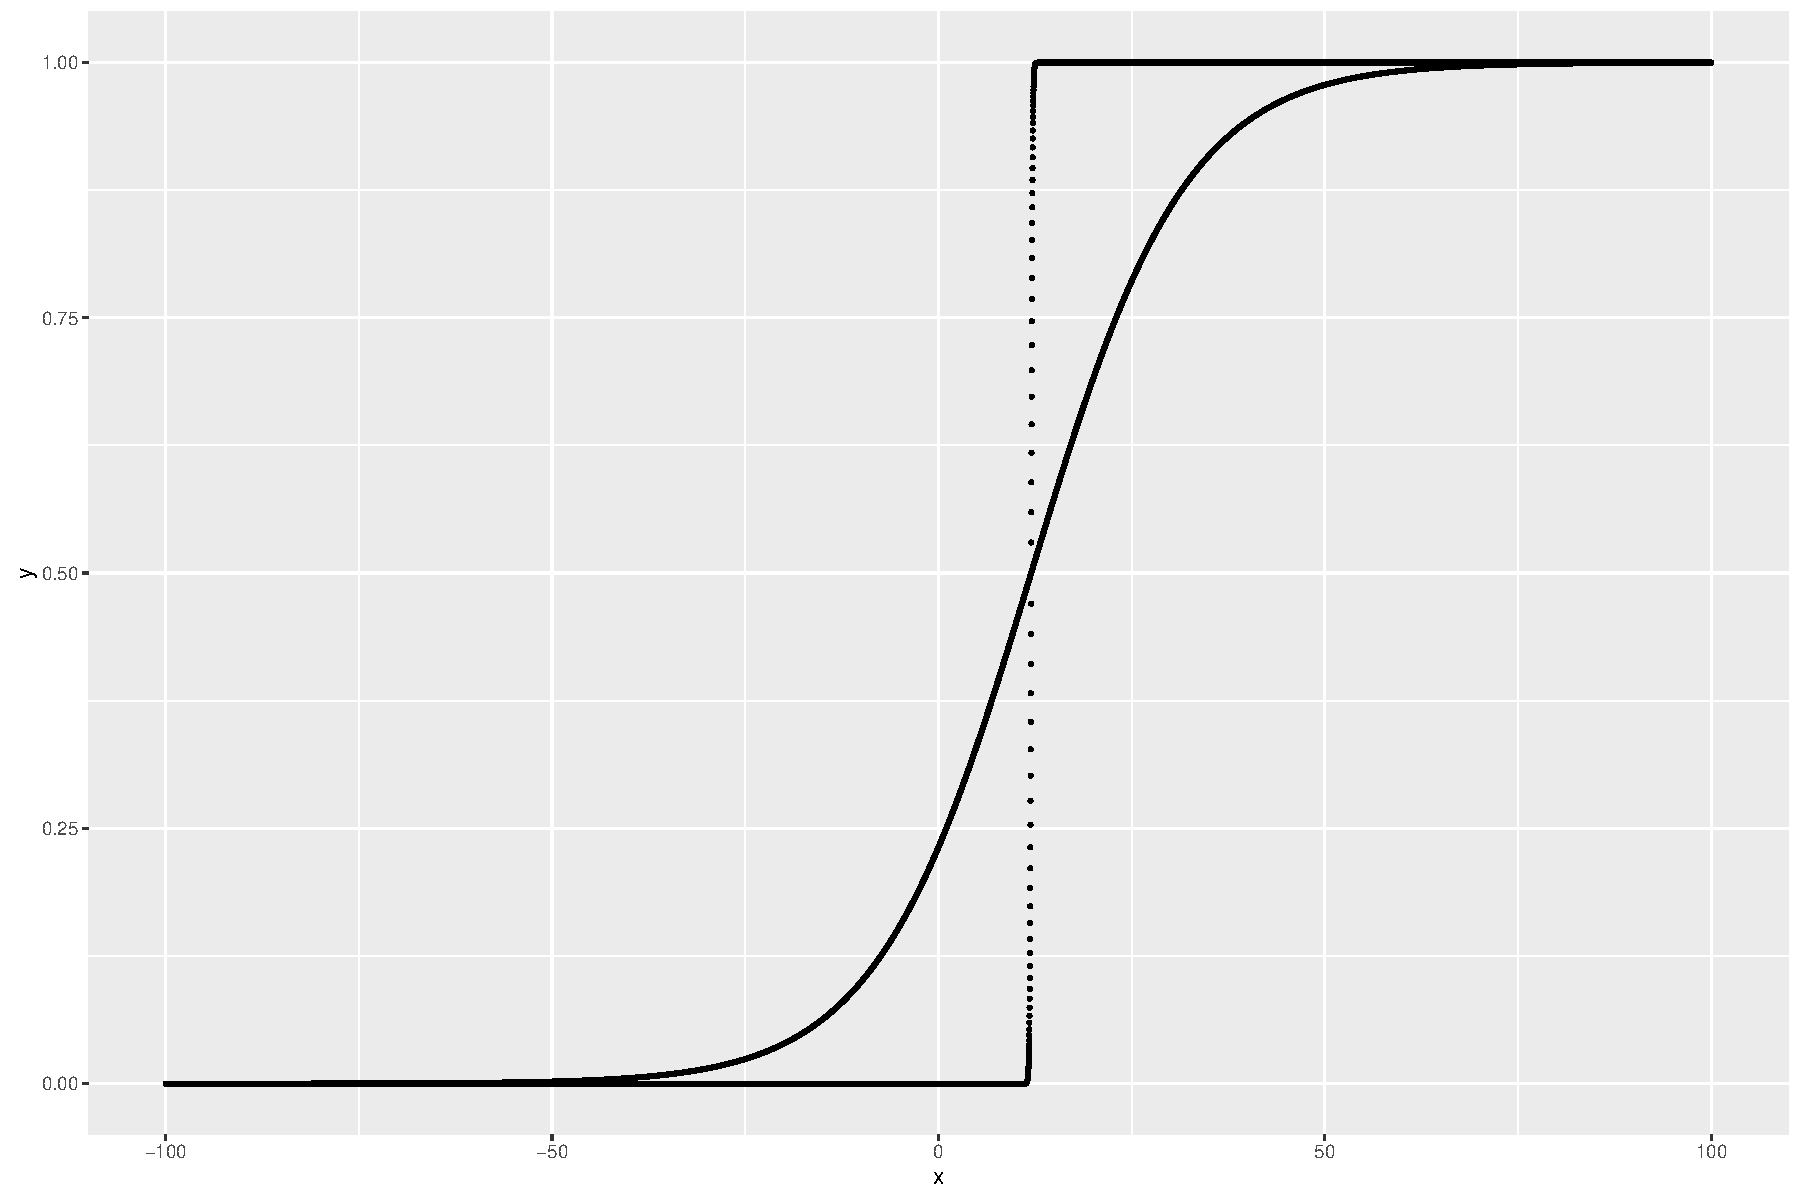
\includegraphics[width=0.9\textwidth]{figure/logistic_curve-1.pdf}
        \caption[Logistic or sigmoid function]{Logistic or sigmoid function for two different values of the parameter $k$}
  \label{fig:logistic_curve}
\end{figure}

The logistic function (shown as Equation \ref{eq:logistic_function} and
as two curves in Figure \ref{fig:logistic_curve}), as we will see, is
very important in many classification and decision settings partly due
to the \emph{non-linear} shape that constrains vertical movement within
the values (0 to 1), and partly because of the range of shapes opened up
by the parameter \(K\). How does a function such as the sigmoid function
`observe' anything? Here the curve itself and even the name `sigmoid' is
the best guide. The S-shape of the sigmoid curve is a good guide to
operations associated with curves. The logistic function has quite a
long history in statistics since that curve diagrams growth and change
in various ways. \index{function!logistic} (As the historian of
statistics J.S. Cramer writes: `The logistic function was invented in
the nineteenth century for the description of the growth of organisms
and populations and for the course of autocatalytic chemical reactions'
\autocite[614]{Cramer_2004}.\footnote{The Belgian mathematician
  Pierre-François Verhulst designated the sigmoid function the `logistic
  curve' in the 1830-40s \autocite[616]{Cramer_2004}. It was
  independently designated the `autocatalytic function' by the German
  chemist Wilhelm Ostwald in the 1880s, and then re-invented under
  various names by biologists, physiologists and demographers during
  1900-1930s (617). The term `logistic' returns to visibility in the
  1920s, and has continued in use as a way of describing the growth of
  something that reaches a limit. \index{logistic function!history of}}
\index{function!logistic!history of} In nearly all of these cases, the
function was used to fit a curve to data on the growth of something:
populations, reactions, tumours, tadpoles tails, oats and embryos. The
reference of the curve to growth comes from its changing slope. Growth
starts slowly, increases rapidly and then slows down again as it reaches
a limit. In the second half of the twentieth century, it was widely used
in economics. In all these settings and usages, the curve was a way of
describing and predicting growth in populations.
\index{population!growth of} Census data, clinical or laboratory
measurements supplied the actual values of \(f(x)\) at particular times,
the \(x\) values. The task of the demographer, physiologist or economist
was to calculate out the values of parameters such as \(k\) that
controlled the shape of the curve.

Historically, then, the logistic function has a well-established
biopolitical resonance. \index{statistics!history!population growth}
\index{biopolitics!populations} But note that the curves showing in
Figure \ref{fig:logistic_curve} plot the same data (\(\mathbf{X}\) and
\(y\) values), but differ in their curvature. This diagrammatic
variation derives from the parameter \(k\), which discreetly appears in
the equation \ref{eq:logistic_function} next to \(x\). Such parameters
are vital control points in function fitting and any learning associated
with that. Varying these parameters and optimising their values is the
basis of `useful approximation' in machine learning.

Sometimes these parameters can be varied so much as to suggest entirely
different functions. \index{function!parameters of} In
\ref{fig:logistic_curve} for instance, \(k=12\) produces a much sharper
curve, a curve that actually looks more like a qualitative change, range
than a smooth transition from \(0\) to \(1\). The sharp shape of the
logistic curve when the scaling parameter \(k\) is larger transforms the
function into a classifier, into a function that, as Breiman puts it, is
equal to one of the numbers \(0\) or \(1\). In this setting, the
function \(f(x) = 1/(1+e^{-x})\) maps continuously varying numbers (the
\(x\) values) onto a domain of discrete values. Because \(f(x)\) tends
very quickly to converge on values of \(1\) or \(0\), it can be coded as
`yes'/`no'; `survived/deceased', or any other binary difference.
\index{differences!binary!sigmoid function} The mapping between the
\(x\) values sliding continuously and the binary difference pivots on
the combination of the exponential function (\(e^{-x}\)), which rapidly
tends towards zero as \(x\) increases and rapidly tends towards
\(\infty\) as \(x\) decreases, and the dividend \(\sfrac{1}{1+ ...}\),
which converts high value denominators to almost zero and low value
denominators to one. This mapping between variations in \(x\) and the
value of the function \(f(x)\) is mathematically elementary, but typical
of the relaying of references that allows functions to intersect with
and constitute matters of fact and states of affairs such as
\texttt{cat} and \texttt{not-cat}. This realisation -- that a
continuously varying sigmoid function can map discrete outcomes -- forms
the basis of many machine learning classifiers.
\index{function!sigmoid|)}

\section{The cost of curves in machine
learning}\label{the-cost-of-curves-in-machine-learning}

\begin{table}[ht]
\centering
\begingroup\tiny
\begin{tabular}{p{0.1\textwidth}p{0.5\textwidth}p{0.3\textwidth}p{0.10\textwidth}}
  \hline
Year & Title & Keywords & Citations \\ 
  \hline
\hline
\end{tabular}
\endgroup
\caption{Sample of highly cited scientific publications referring to "logistic regression" in title or keyword} 
\label{tab:logistic_in_ml}
\end{table}

I have been suggesting that experimentality in machine learning consists
in coupling operational and observational functions. If operational
functions move through or transform the data, observational functions
render the effects of those transformations visible. How does this take
place practically? The logistic function appears frequently in machine
learning literature, prominently as part of perhaps the most vernacular
machine learner, the logistic regression model (see table
\ref{tab:logistic_in_ml} for a sample of well-cited publications).
\index{machine learner!logistic regression} Descriptions of logistic
regression models appear in nearly all machine learning tutorials,
textbooks and training courses (see Chapter 4 in
\autocite{Hastie_2009}). \index{science!biomedicine!machine learners in}
In biomedical research, `logistic regression is the default ``simple''
model for predicting a subject's group status'
\autocite[43]{Malley_2011}. As Malley et.al. suggest, `it can be applied
after a more complex learning machine has done the heavy lifting of
identifying an important set of predictors given a very large list of
candidate predictors' (43). Especially in comparison to more complicated
models, logistic regression models are relatively easy to interpret
because they are superimpose the logistic function on the linear model
that we have been discussing already (see figure
\ref{fig:linreg_classifier_hastie} and also chapters \ref{ch:diagram}
and \ref{ch:vector}). As \emph{Elements of Statistical Learning} puts
it: `the logistic regression model arises from the desire to model the
posterior probabilities of the \(K\) classes via linear functions in
\(x\), while at the same time ensuring that they sum to one and remain
in \([0,1]\)' \autocite[119]{Hastie_2009}. The logistic regression model
predicts what class or category a particular instance is likely to
belong to, but `via linear functions in \(x\).'

We see something of this predictive desire from the basic mathematical
expression for logistic regression in a situation where there are binary
responses or \(K=2\):

\begin {equation}
\label {eq:logistic_regression}
Pr(G=K|X=x) = \frac{1}{1+e^{\sum_{l=1}^{K-1}(\beta_{l0} + \beta_l^Tx)}} 
\end {equation}

\autocite[119]{Hastie_2009}

Equation \ref{eq:logistic_regression} encapsulates lines in curves. That
is, the linear model (the model that fits a plane to a scattering of
points in vector space) appears as \(\beta_l0 + \beta_l^Tx\), where as
usual \(\beta\) refers to the parameters of the model and \(x\) to the
matrix of input values. The linear model has, however, now been relayed
through the sigmoid function so that its output values no longer
increase and decrease linearly. Instead they follow the curve of the
logistic function, and range between a minimum of \(0\) and a maximum of
\(1\), a range of values that map onto probabilities (as discussed in
the next chapter \ref{ch:probability}. As usual, small typographic
conventions diagram some of this transformation.
\index{diagrammatic!transformation} In equation
\ref{eq:logistic_regression}, some new characters appears: \(G\) and
\(K\). Previously, the response variable, the variable the model is
trying to predict, appeared as \(Y\). \index{data!variable!response}
\(Y\) refers to a continuous value whereas \(G\) refers to membership of
a group or class (e.g.~survival vs.~death; male vs female;
etc.).\footnote{What does this wrapping of the linear model in the curve
  of the sigmoid logistic curve do in terms of finding a function? Note
  that the shape of this curve has no intrinsic connection or origin in
  the data. The curve no longer corresponds to growth or change in size,
  as it did in its nineteenth century biopolitical application to the
  growth of populations. Rather, the curvilinear encapsulation of the
  linear model allows the left hand side of the expression to move into
  a different register. The left hand side of the expression is now a
  probability function, and defines the probability (\(Pr\)) that a
  given response value (\(G\)) belongs to one of the pre-defined classes
  (\(k = 1, ..., K-1\)). In this case, there are two classes (`yes/no'),
  so \(K=2\). Unlike linear models, that predict continuous \(y\) values
  for a given set of \(x\) inputs, the logistic regression model
  produces a probability that the instance represented by a given set of
  \(x\) values belongs to a particular class. When logistic regression
  is used for classification, values greater than \(0.5\) are usually
  read as class predictions of `yes', `true' or \texttt{1}. As a result,
  drawing lines through the vector space can effectively become a way of
  classifying things. Note that this increase in flexibility comes at
  the cost of a loss of direct connection between the data or features
  in the generalized vector space, and the output, response or predicted
  variables. They are now connected by a mapping that passes through the
  somewhat more mobile and dynamic operation of exponentiation \(exp\),
  a function whose rapid changes can be mapped onto classes and
  categories.}

\section{Curves and the variation in
models}\label{curves-and-the-variation-in-models}

Whether or not the logistic function is a useful approximation to `the
function that underlies the predictive relationship between input and
out' depends on how it relates input and output. The way in which we
have `learned' the logistic function by taking a textbook formula
expression of it, and plotting the function associated with it is not
the way that machine learners typically `learns' an approximation to the
predictive relationship between the input data and the output or
`response variable'. For a machine learner, finding a function means
optimising function parameters on the basis of the data not deriving a
formula. Machine learning is not a matter of mathematical analysis, but
of algorithmic optimisation.\footnote{Even in machine learning, some
  function-finding through solving systems of equations occurs. For
  instance, the closed form or analytical solution of the least sum of
  squares problem for linear regression is given by
  \(\hat{\beta} = (\mathbf{X}^T\mathbf{X})^{-1}\mathbf{X}^T\mathbf{y}\).
  \index{mathematics!closed form solutions} As we saw in the previous
  chapter, this expression provides a very quick way to calculate the
  parameters of a linear model given a matrix of input and output
  values. This formula itself is derived by solving a set of equations
  for the values \(\hat{\beta}\), the estimated parameters of the model.
  But how do we know whether a model is a good one, or that the function
  that a model proffers to us fits the functions in our data, or that it
  `minimises the probability of error'? One problem with closed-form or
  analytical solutions typical of mathematical problem-solving is
  precisely that their closed-form obscures the algorithmic processes
  needed to actually compute results. The closed form solution estimates
  the parameters of the linear model by carrying out a series of
  operations on matrices of the data. These operations include matrix
  transpose, several matrix multiplications (so-called `inner product')
  and matrix inversion (the process of finding a matrix that when
  multiplied by the input matrix yields the identity matrix, a matrix
  with \(1\) along the diagonal, and \(0\) for all other values). All of
  these operations take place in the vector space. When the dataset,
  however, has a hundred or a thousand rows, these operations can be
  implemented and executed easily. But as soon as datasets become much
  larger, it is not easy to actually carry out these matrix operations,
  particularly the matrix inversion, even on fast computers. For
  instance, a dataset with a million rows and several dozen columns is
  hardly unusual today. Although linear algebra libraries are carefully
  crafted and tested for speed and efficiency, closed form solutions,
  even for the simplest possible structures in the data, begin to break
  down. \index{vector space!matrix operations}}
\index{parameters!optimisation of} \index{optimisation}
\index{machine learning!optimisation in}

If we turn just to the diagrammatic forms associated with logistic
regression in \emph{Elements of Statistical Learning}, something quite
different and much more complicated than calculating the values of a
known function presents itself there. For instance, in their analysis of
the \texttt{South\ African\ coronary\ heart} disease data, Hastie and
co-authors repeatedly model the risk of occurrence of heart disease
using logistic regression. \index{dataset!South African Heart Disease}
They first apply logistic regression fitted by `maximum likelihood', and
then by `L1 regularized logistic regression'
\autocite[126]{Hastie_2009}. The results of this function-finding work
appear as tables of coefficients or as `regularization plots.' As is
often the case, \emph{Elements of Statistical Learning} assumes that
readers already understand conventional statistical usages of logistic
regression. Discussion dwells instead on observing how values of the
model parameter change as different variants of the model transform the
data.

\begin{verbatim}
## Error in library(ElemStatLearn): there is no package called 'ElemStatLearn'
\end{verbatim}

\begin{verbatim}
## Error in library(glmnet): there is no package called 'glmnet'
\end{verbatim}

\begin{verbatim}
## Error in factor(SAheart$chd): object 'SAheart' not found
\end{verbatim}

\begin{verbatim}
## Error in as.matrix(SAheart[, c("sbp", "ldl", "adiposity", "typea", "obesity", : object 'SAheart' not found
\end{verbatim}

\begin{verbatim}
## Error in eval(expr, envir, enclos): object 'SAheart' not found
\end{verbatim}

\begin{verbatim}
## Error in eval(expr, envir, enclos): object 'SAheart' not found
\end{verbatim}

\begin{verbatim}
## Error in ylim[1]: object of type 'closure' is not subsettable
\end{verbatim}

\begin{verbatim}
## Error in xlim[1]: object of type 'closure' is not subsettable
\end{verbatim}

\begin{verbatim}
## Error in expand.grid(xtmp, ytmp): object 'xtmp' not found
\end{verbatim}

\begin{verbatim}
## Error in eval(expr, envir, enclos): could not find function "glmnet"
\end{verbatim}

\begin{verbatim}
## Error in predict(SAheart_model2, as.matrix(newx), type = "class", s = 0.001): object 'SAheart_model2' not found
\end{verbatim}

\begin{verbatim}
## Error in data.frame(x = rep(xtmp, length(ytmp)), y = rep(ytmp, each = length(xtmp)), : object 'xtmp' not found
\end{verbatim}

\begin{verbatim}
## Error in ggplot(data = SAheart, aes(x = sbp, y = ldl)): object 'SAheart' not found
\end{verbatim}

\begin{verbatim}
## Error in eval(expr, envir, enclos): object 'g' not found
\end{verbatim}

\begin{verbatim}
## Error in eval(expr, envir, enclos): object 'g' not found
\end{verbatim}

\begin{verbatim}
## Error in eval(expr, envir, enclos): could not find function "glmnet"
\end{verbatim}

\begin{verbatim}
## Error in plot(SAheart_model2): object 'SAheart_model2' not found
\end{verbatim}

\begin{verbatim}
## Error in summary(SAheart_model2): object 'SAheart_model2' not found
\end{verbatim}

\begin{verbatim}
## Error in print(tab2): object 'tab2' not found
\end{verbatim}

\begin{figure}
      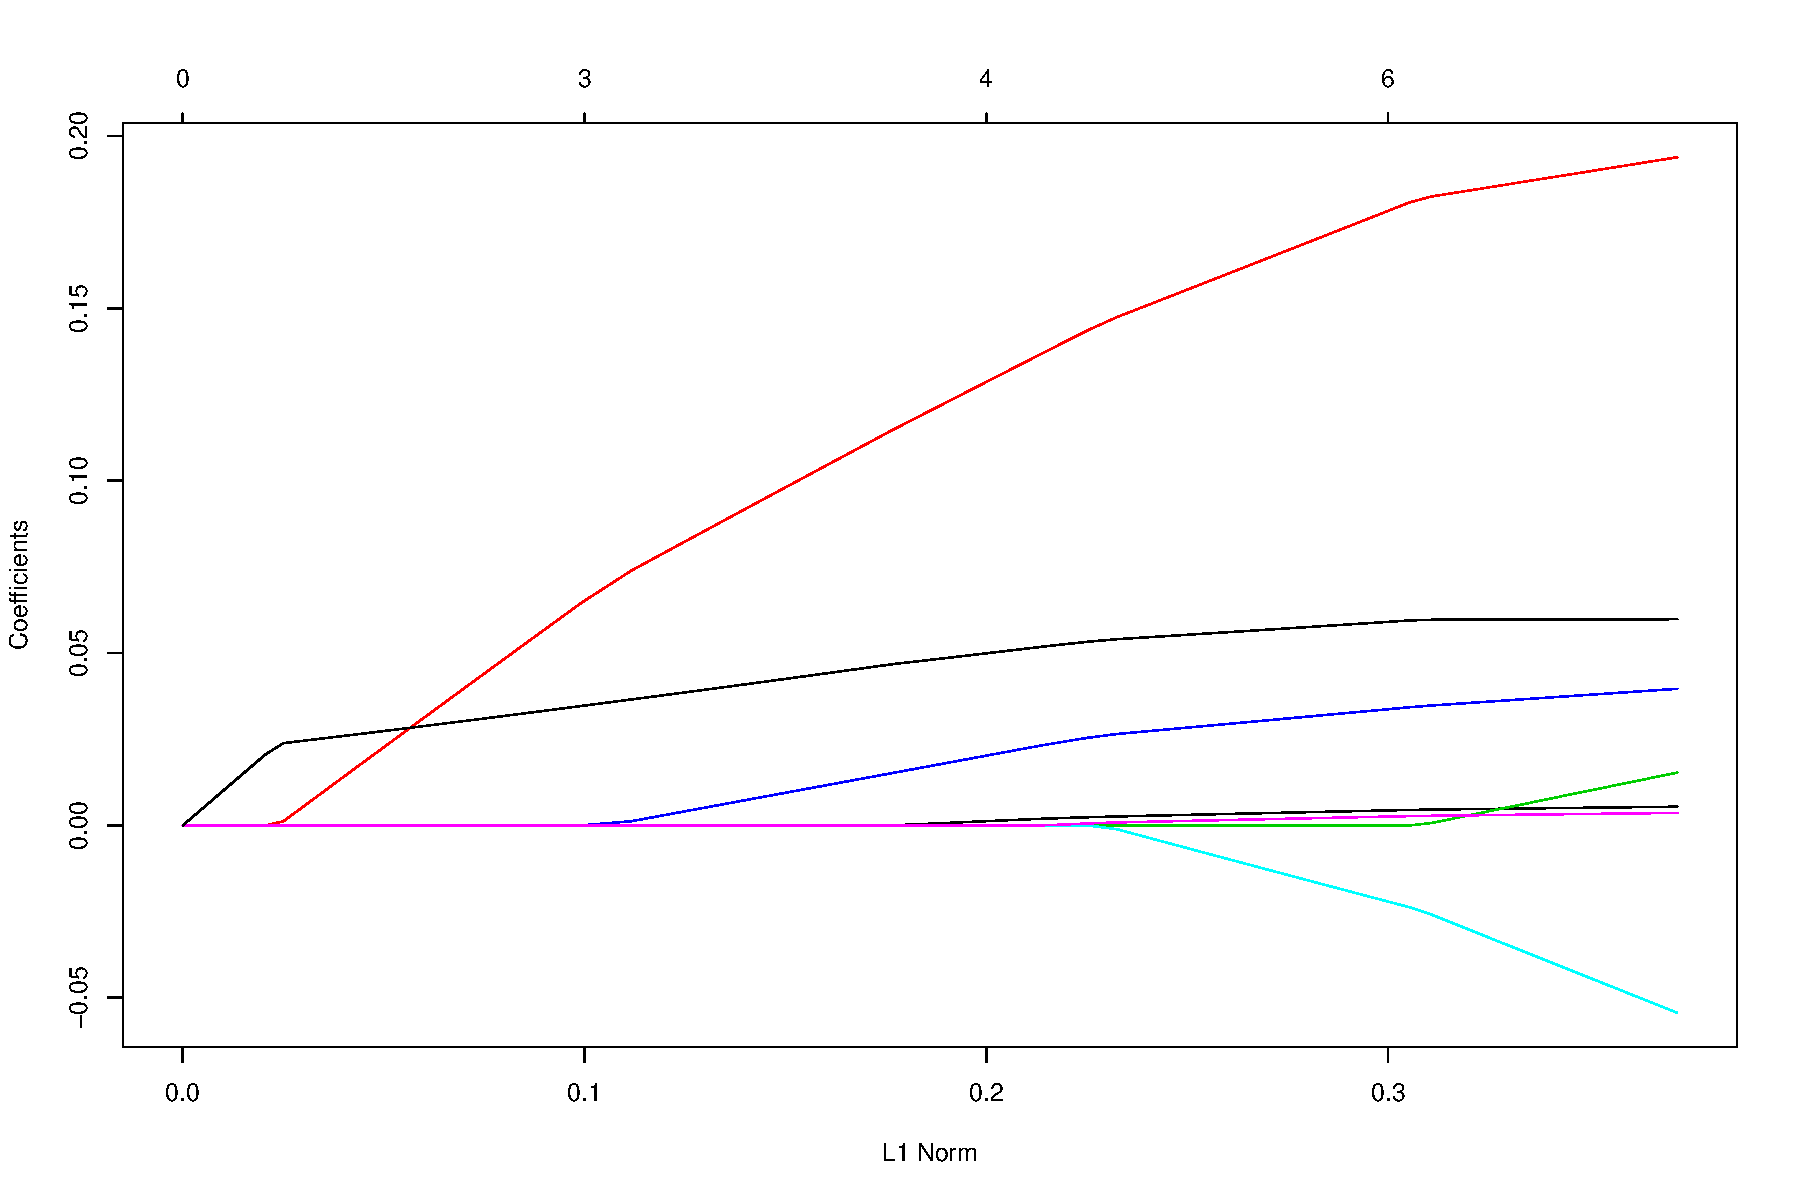
\includegraphics[width=0.9\textwidth]{figure/sa_heart_model-2.pdf}
        \caption{South African Heart disease regularization plot}
  \label{fig:heart_model}
\end{figure}

\begin{figure}
  \centering
      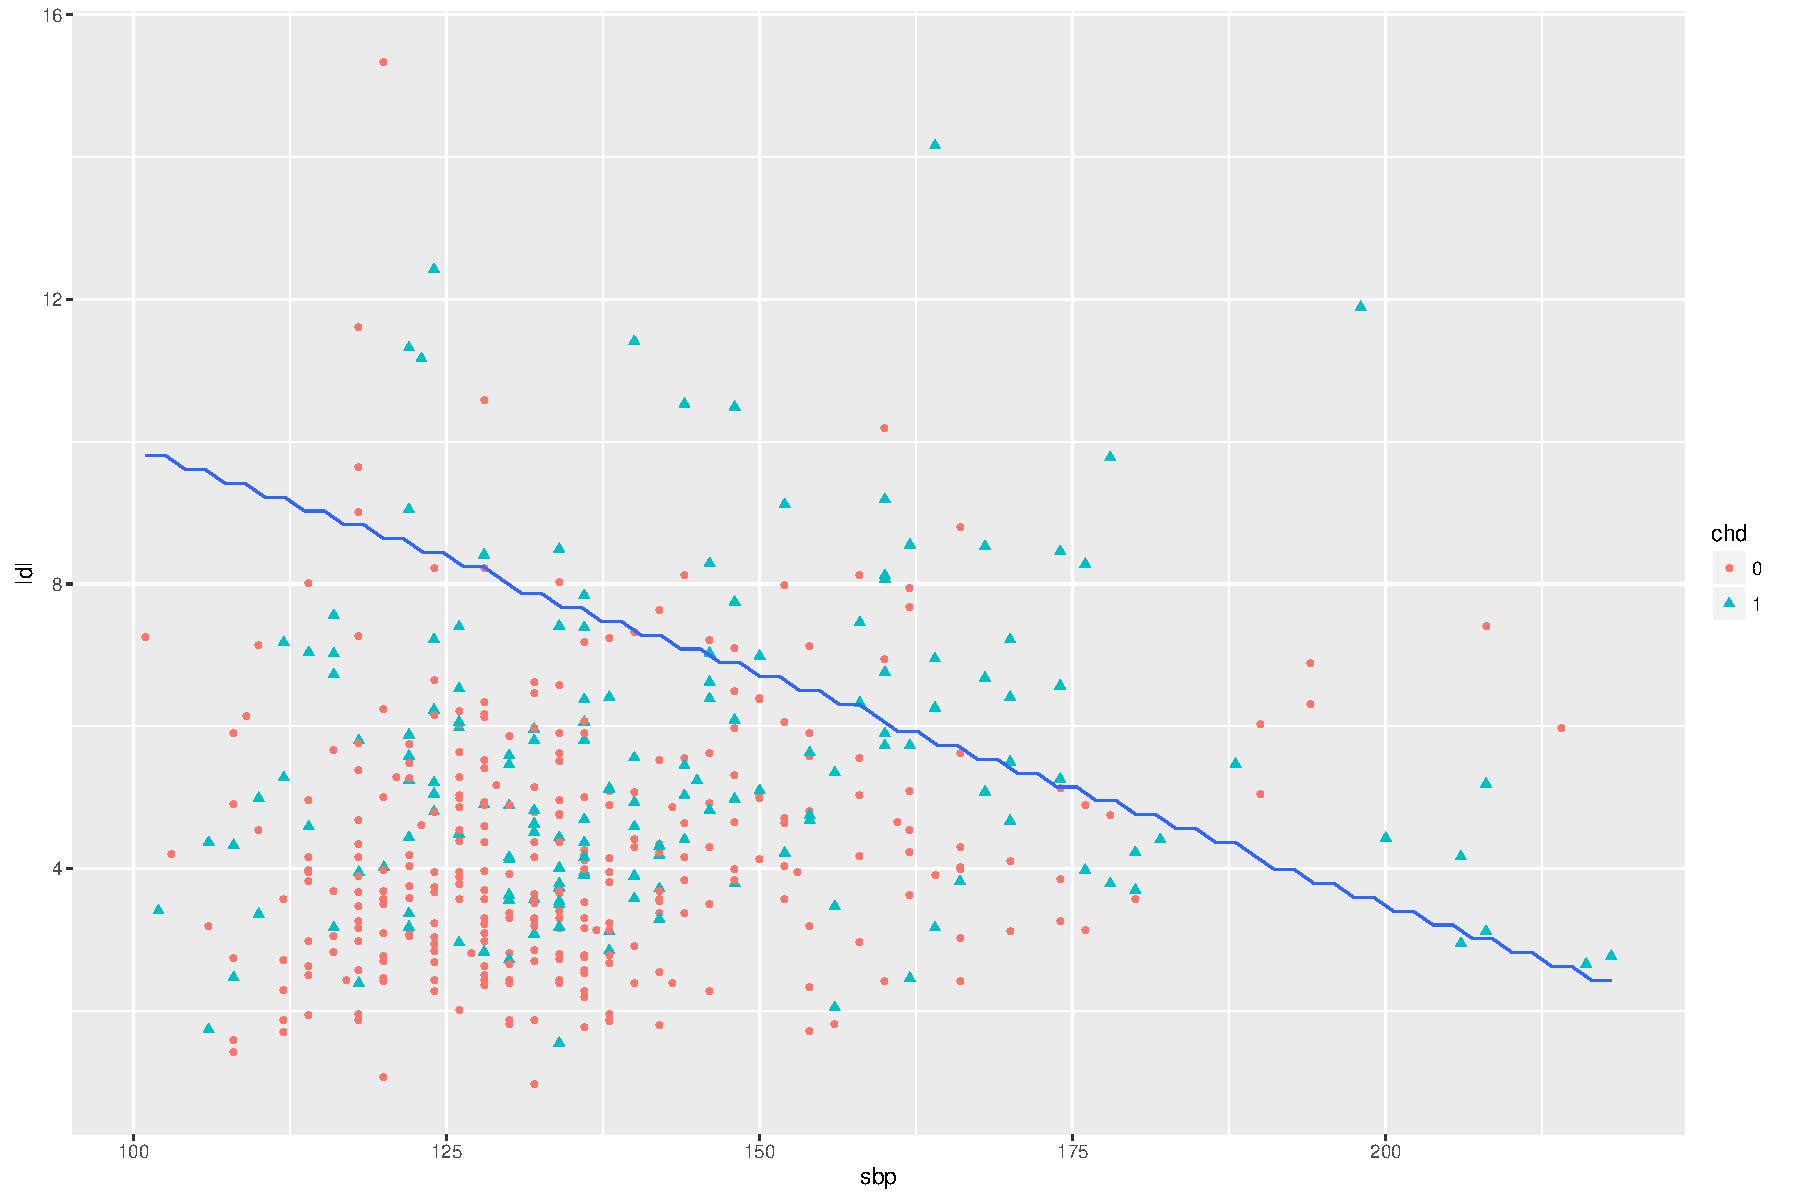
\includegraphics[width=0.9\textwidth]{figure/sa_heart_model-1.pdf}
        \caption{South African Heart disease decision plane}
  \label{fig:heart_plane}
\end{figure}

Figure \ref{fig:heart_model} shows a series of lines. Plotted after the
model transforms the data 366 times, each line sets out the changing
importance of a particular variable --
\texttt{obesity,\ alcohol\ consumption,\ weight,\ age,} designated by
numbers shown on the right hand side -- as it is included in the
logistic regression model in a different way. The learning or
function-finding diagrammed in figure \ref{fig:heart_model} concerns
variations in parameters and ways of automating the variation of
parameters beyond that undertaken by modelling experts such as
statisticians and scientists when they fit models to data. \footnote{As
  we saw in chapter \ref{ch:vector}, the production of new tables of
  numbers that list the parameters of models actually transform the
  vectorised data into new subspaces (a line, plane, a surface).
  \index{vectorisation} Many of the plots and tables found in machine
  learning texts, practice and code offer nothing else but measurements
  of how the model parameters weight slightly different transformations
  of the vector space. In the case of logistic regression, the shape of
  the curve is determined using maximum likelihood. For present
  purposes, the statistical significance of this procedure is less
  important than the algorithmic implementation. This is the opposite to
  what might appear in a typical statistics textbook where the
  implementation of maximum likelihood would normally be quickly passed
  over. For instance, in \emph{An Introduction to Statistical Learning
  with R}, a textbook focused on using \texttt{R} to implement machine
  learning techniques, the authors write: `we do not need to concern
  ourselves with the details of the maximum likelihood fitting
  procedure' \autocite[133]{James_2013}.
  \index{maximum likelihood!implementation of}}
\index{parameters!variation of}

We saw that the classic statistical model of linear regression fits
lines to the data through the linear algebra method of ordinary least
squares (see chapter \ref{ch:vector}, equation
\ref{eq:linear_model_solution}). Several obstacles hinder the
construction of models using closed form approximate solutions. Unique
`closed form' or analytical solutions are quite unusual in machine
learning. While they do exist for linear regression, they don't exist
for logistic regression nor for more complex machine learners. Equally
problematically, the closed form solution is run once, and the model it
produces is subject to no further variation. The parameters define the
line of best fit. It can be interpreted by the modeller in terms of
\emph{p} or \(R^2\) or other measures of the model's fit. But the model
itself does not generate variations. \footnote{As soon as we move from
  the more theoretical or expository accounts of function-finding into
  the domain of practice, instruction and learning of machine learning,
  a second sense of function comes to the fore. The second sense of
  function comes from programming and computer science. A function there
  is a part of the code of a program that performs some operation, `a
  self-contained unit of code,' as Derek Robinson puts it
  \autocite[101]{Robinson_2008}.
  \index{function!operational!unit of code} The three lines of R code
  written to produce the plot of the logistic function are almost too
  trivial to implement as a function in this sense, but they show
  something of the transformations that occur when mathematical
  functions are operationalised in algorithmic form. The function is
  wrapped in a set of references. First, the domain of \(x\) values is
  made much more specific. The formulaic expression
  \(f(x) = 1/(1+e^{-x})\) says nothing explicitly about the \(x\)
  values. They are implicitly real numbers (that is,
  \(x \in \mathbb{R}\)) in this formula but in the algorithmic
  expression of the function they become a sequence of 20001 generated
  by the code. Second, the function itself is flattened into a single
  line of characters in code, whereas the typographically the
  mathematical formula had spanned 2-3 lines. Third, a key component of
  the function \(e^-x\) itself refers to Euler's number \(e\), which is
  perhaps the number most widely used in contemporary sciences due to
  its connection to patterns of growth and decay (as in the exponential
  function \(e^x\) where \(e = 2.718282\) approximately). This number,
  because it is `irrational,' has to be computed approximately in any
  algorithmic implementation.}

\section{Observing costs, losses and objectives through
optimisation}\label{observing-costs-losses-and-objectives-through-optimisation}

Faced with the impracticality of an analytical or mathematically closed
form solution to the problem of finding a function, machine learners
typically seek ways of observing how different models traverse the data.
They replace the exactitude and precision of mathematically-deduced
closed-form solutions with algorithms that generate varying solutions. A
range of techniques search for optimal combinations of parameters. These
optimisation techniques are the operational underpinning of machine
learning. \index{machine learning!optimisation} Without their iterative
processes, there is no machine in machine learning. They have names such
as `batch gradient descent', `stochastic gradient ascent,' `coordinate
descent,' `coordinate ascent' as well as the `Newtown-Raphson method' or
simply `convex optimisation' \autocite{Boyd_2004}.
\index{algorithm!gradient descent} These techniques have a variety of
provenances (Newton's work in the 17th century, for instance, but more
typically fields such as operations research that were the focus of
intense research efforts during and after World War ; see
\autocites{Bellman_1961}{Petrova_1997}{Meza_2010}). Much of the learning
in machine learning occurs through these somewhat low-profile yet
computationally intensive techniques of optimisation.
\index{optimisation!history of}

Optimisation is a practice of observation. `Science brings to light
partial observers in relation to functions within systems of reference'
write Gilles Deleuze and Félix Guattari in their account of scientific
functions \autocite[129]{Deleuze_1994}.\footnote{Its hard to know
  whether Deleuze and Guattari were aware of the extensive work done on
  problems of mathematical optimization during the 1950-1960s, but their
  strong interest in the differential calculus as a way of thinking
  about change, variation and multiplicities somewhat unexpectedly makes
  their account of functions highly relevant to machine learning.
  \index{Deleuze, Gilles!calculus}} \index{function!as partial observer}
\index{Deleuze, Gilles!on functions}\index{Guattari, Félix!on functions}
In many machine learning techniques, the search for an approximation to
the function that generated the data is optimised by reference to
another function called the `cost function' (also known as the
`objective function' or the `loss function'; the terms are somewhat
evocative of both economics and cybernetics). Machine learning problems
are framed in terms of minimizing or maximising the cost function.
\index{function!cost, loss or objective} `Cost' or `loss' takes the form
of errors, and minimizing the cost function implies minimizing the
number of errors made by a machine learner. As we saw earlier, in his
formulation of the `learning problem', the learning theorist Vladimir
Vapnik speaks of choosing a function that approximates to the data, yet
minimises the `probability of error' \autocite[31]{Vapnik_1999}.

The \gls{cost function} compares predictions generated by a machine
learner to known values in the data set. Every cost function implies
some measure of the difference or distance between the prediction and
the values actually measured. Cost functions in common use include
squared error, hinge loss, log-likelihood and cross-entropy.
\index{function!cost!variety of} In classifying outcomes into two
classes (the patient survives versus patient dies; the user clicks
versus user doesn't click; etc.), the cost function has to express their
either/or outcome. Crucially, if cost functions re-configure `the act of
fitting a model to data as an optimization problem'
\autocite[183]{Conway_2012}, function finding and hence machine learning
in general occurs iteratively. Given a cost function, a machine learner
can vary its parameters keeping in view -- or partially observing --
whether the cost function increases or decreases. Just as the logistic
function wraps the linear regression model in a sigmoid curve that
switches smoothly between binary values, the cost functions diagram
model parameters (usually noted as \(\beta\)) in relation to known
responses or output values in the data. If there is learning here, it
does derive from mathematic forms or higher abstraction. Cost functions
diagram relations between models, and render their predictive reference
through the negative feedback loops described by Norbert Wiener
\autocite{Wiener_1961}. \index{optimisation!as negative feedback}
\index{Wiener, Norbert!feedback} Importantly, these feedback loops are
not closed mechanisms but places from which variations can be viewed.
\index{machine learner!learning of}

For instance, the log-likelihood function,
\index{function!cost!log-likelihood|(} a typical and widely-used cost
function associated with logistic regression is defined as:

\begin{equation}
\label {eq:cost_function_logreg}
J(\beta) = \sum_{i=1}^{m} y_i log{ h(x_i)} + (1 -  y_i) log{(1 - h(x_i)})
\end{equation}

where

\[h_{\beta}(x) = \frac{1}{1+e^{-\beta^T x}}\]

Equation \ref{eq:cost_function_logreg} enfolds several manipulations and
conceptual framings (particularly the Principle of Maximum Likelihood, a
statistical principle; see chapter \ref{ch:probability}). But key terms
stand out. First, the cost function \(J(\beta)\) is a function of all
the parameters (\(\beta\)) of the model. They substitute in through the
subsidiary function \(h_{\beta}(x)\), the logistic function function
encapsulating a linear function \(\beta^T X\) . Second, the function
defines a goal of maximising the overall value of the expression,
\(J(\beta)\) as a function of variations in the parameters \(\beta\).
The \(min\) describes the results of the repeated application of the
function. Third, the heart of the cost function is balancing of two
tendencies: it adds (\(\sum\)) all the values where the probability of
the predicted class of a particular case \(h(x_i)\) matches the actual
class \(y_i\), and subtracts (\(1-y\)) all the cases where the
probability of the predicted class does not match the actual class. This
so-called \emph{log likelihood} function can be maximised through
optimisation, but not solved in closed form. The optimal values for
\(\beta\), the model parameters that define the model function need to
be found through some kind of search.
\index{function!cost!log-likelihood|)}

\section{Gradients as partial
observers}\label{gradients-as-partial-observers}

We have some sense of how a function can be configured as an observer,
but little sense of how they manage variations. Many optimization
techniques rely on differential calculus and particularly the calculus
of variations to maximise or minimise the value of a cost function. In
fact, loss functions are often chosen on the basis of their
differentiability. \index{mathematics!differential calculus!variations}
One widely used optimisation algorithm called `gradient descent' is
quite easy to grasp intuitively. In neural nets and deep learning,
gradient descent (or ascent) occurs on an increasingly vast scale.
\index{gradient descent|see {optimisation!gradient descent}} As in many
formulations of machine learning techniques, the framing of the problem
is finding the parameters of the model/function that best approximates
to the function that generated the data. It optimises the parameters of
a model by searching for the maximum or minimum values of the objective
function. The algorithm can be written using calculus style notation as:

\begin{equation}
\label{eq:stochastic_gradient_ascent}
Repeat until convergence:
\beta_{j} := \beta_j + \alpha (y_i - h_\beta(x_i))x_{\beta j}
\end{equation}

The version of the algorithm shown in algorithm
\ref{eq:stochastic_gradient_ascent} is called `stochastic gradient
descent.' Archaeologically, in presenting such formula, the point is not
to read and understand them directly but to characterise the enunciative
function that regulates them. Practical understanding would be the point
in a machine learning course.\index{mathematics!equation!as diagram}
Actually reading these formal expressions, and being able to follow the
chain of references, and indexical signs that lead away from them in
various directions depends very much on the diagrammatic processes
described in chapter \ref{ch:diagram}. Many people who directly use
machine learning techniques in industry and science would not often if
ever need to make use of such expressions as they build models. They
would mostly take them for granted, and simply execute via functions
supplied by software libraries (e.g. \texttt{GradientDescentOptimizer}
in the \texttt{TensorFlow} library or \texttt{StochasticGradient} in
\texttt{torch}).\index{optimisation!gradient descent!stochastic}

\begin{figure}
  \centering
      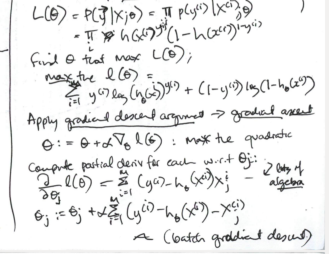
\includegraphics[width=0.9\textwidth]{figure/log_reg_stochastic_ascent.pdf}
        \caption{Gradient ascent for logistic regression}
  \label{fig:gradient_ascent}
\end{figure}

Given that equation \ref{eq:stochastic_gradient_ascent} encapsulates the
heart of a major optimisation technique, we might first of all be struck
by its operational brevity. This is not an elaborate or convoluted
algorithm. As Malley, Mally and Pajevic observe, `most of the {[}machine
learning{]} procedures \ldots{} are (often) nearly trivial to implement'
\autocite[6]{Malley_2011}. Note that this expression of the algorithm,
taken from the class notes for {[}Lecture 3{]} of Andrew Ng's `Machine
Learning' CS229 course at Stanford (\autocite{Ng_2008j}; see figure
\ref{fig:gradient_ascent}), mixes an algorithmic set of operations with
function notation. We see this in several respects: the formulation
includes the imperative `repeat until convergence'; it also uses the
so-called `assignment operator' \(:=\) rather than the equality operator
\(=\). The latter specifies that two values or expressions are equal,
whereas the former specifies that the values on the right hand side of
the expression should be assigned to the left. Both algorithmic forms --
repeat until convergence, and assign/update values -- owe more to
techniques of computation than to mathematical abstraction.

\begin{figure}
  \centering
      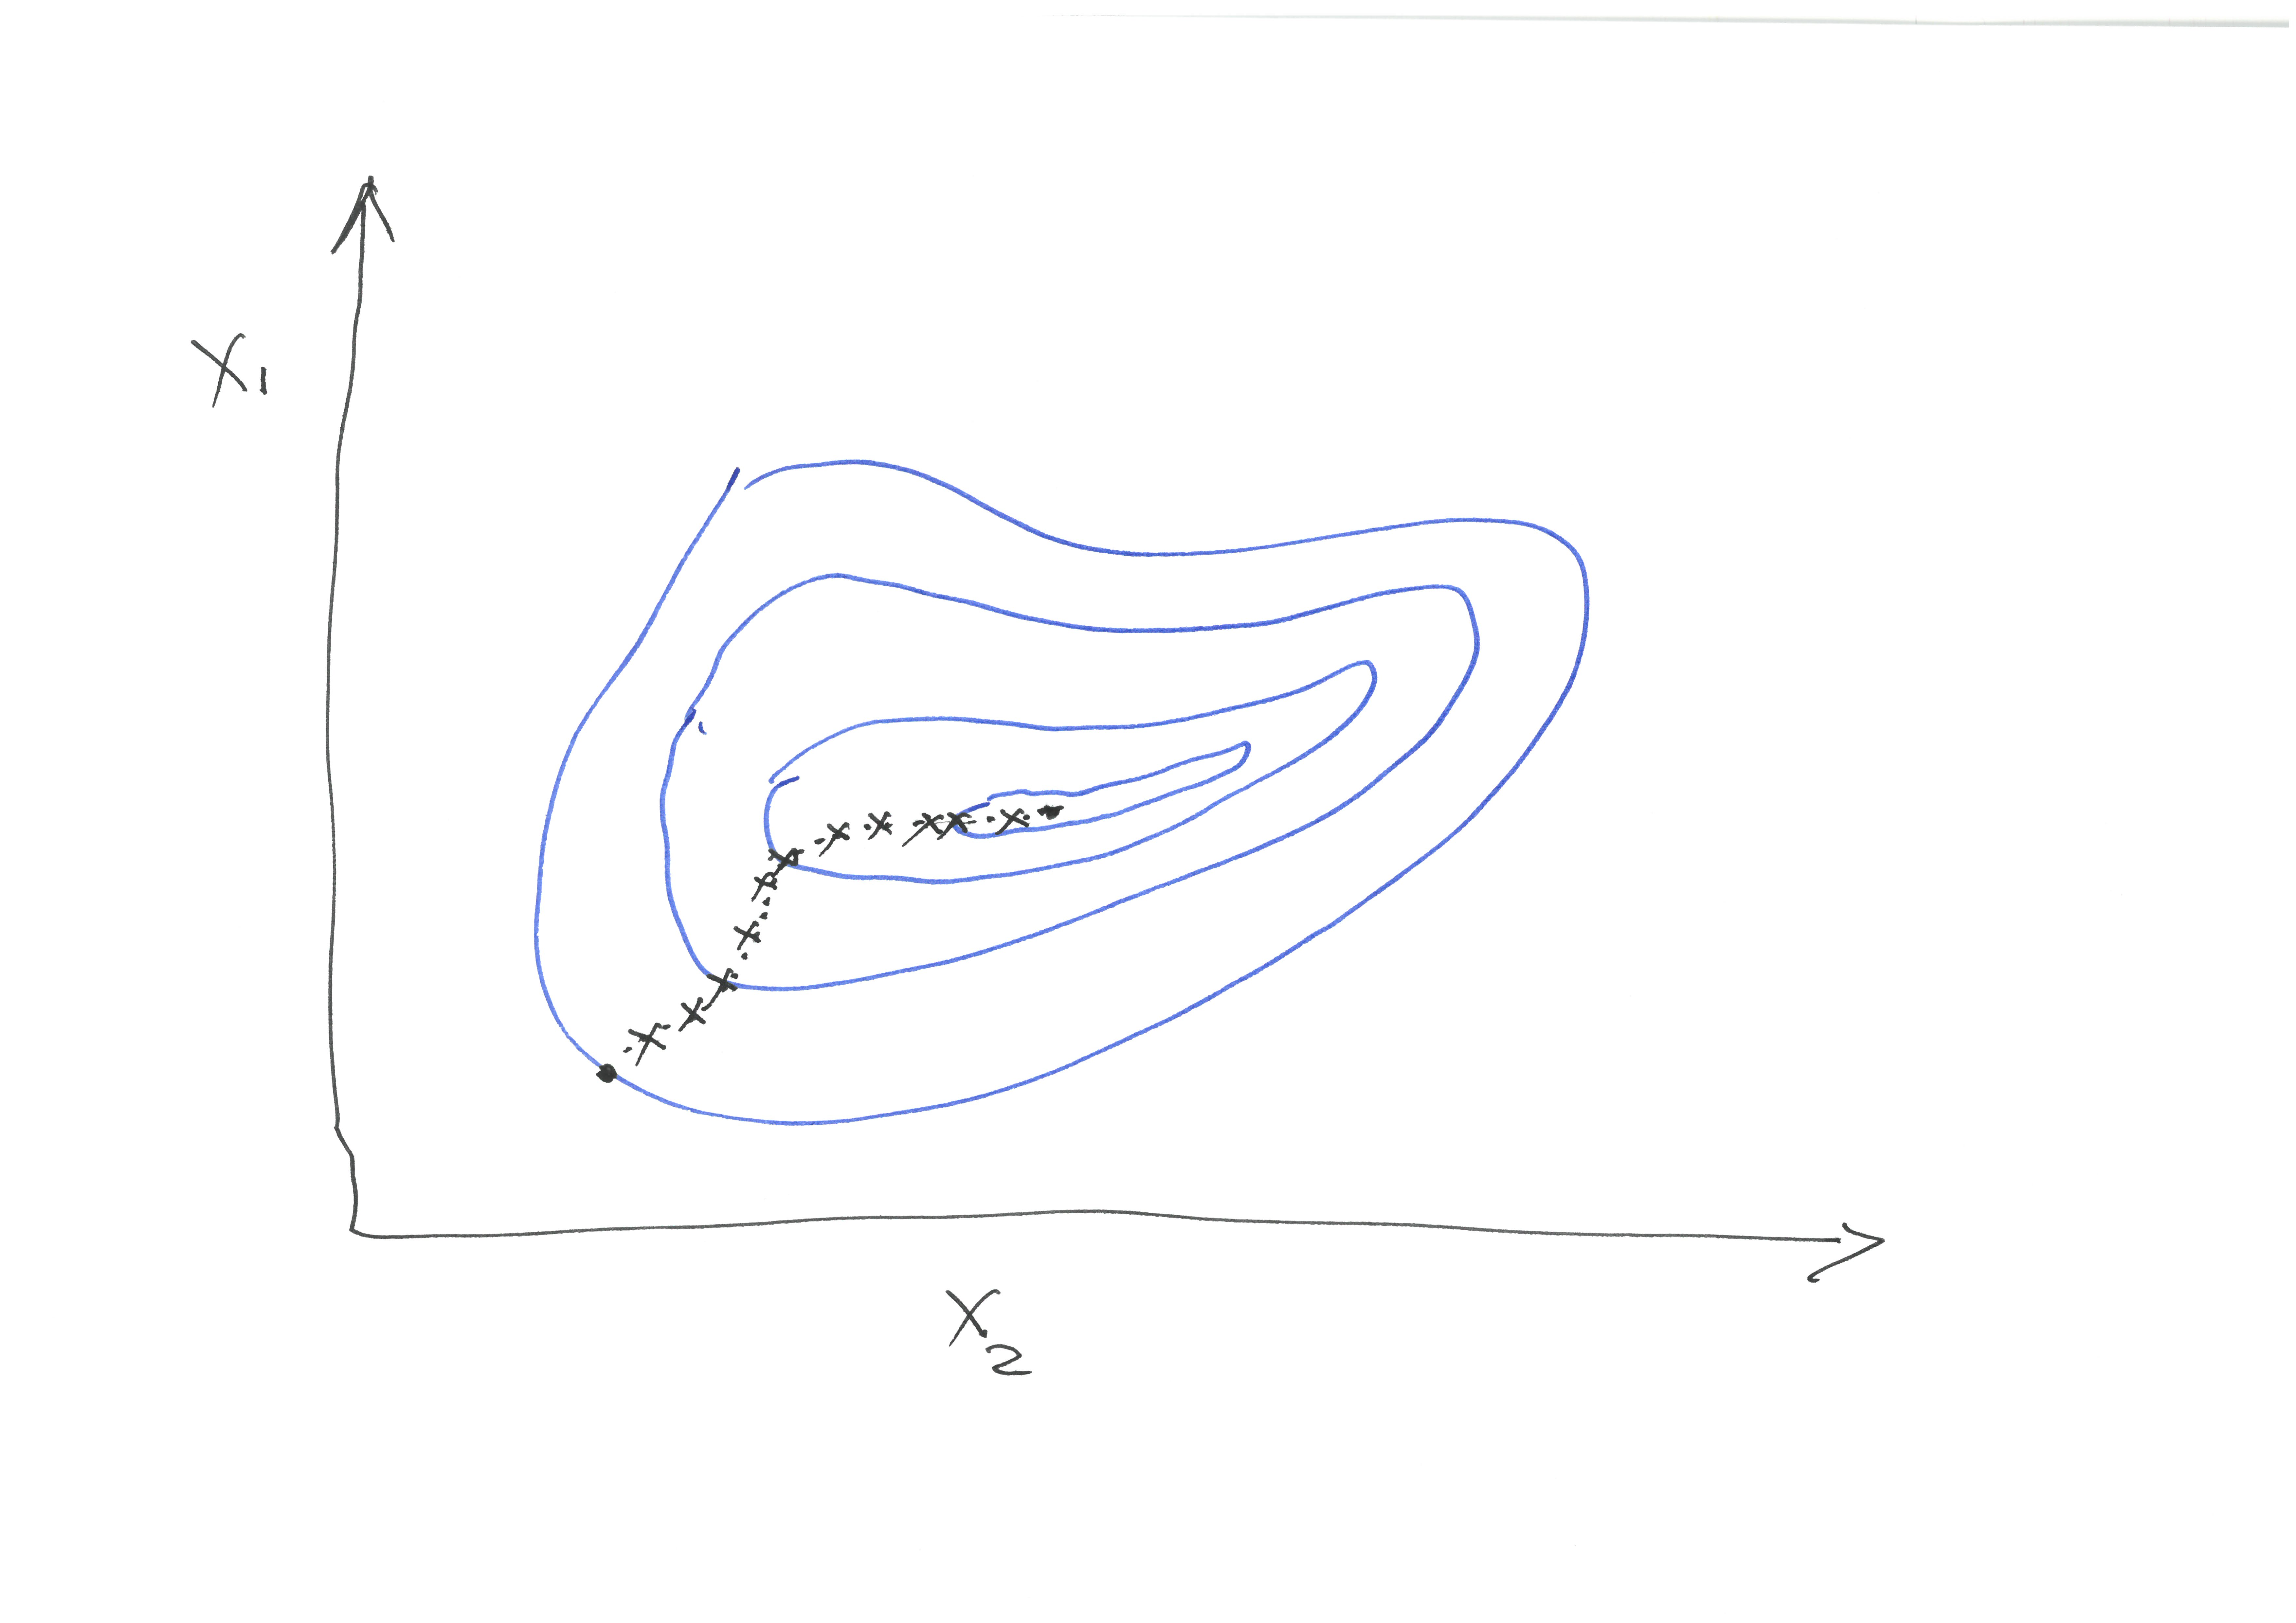
\includegraphics[width=0.9\textwidth]{figure/stochastic_gradient_handdrawn.jpg}
        \caption{Stochastic gradient descent path}
  \label{fig:stoch_grad_hand}
\end{figure}

In gradient descent, we see functions acting as partial observers. The
specification for the gradient descent algorithm brings us to the scene
where ongoing transformation of data from irregular volume to plane can
be observed. At the heart of this reshaping lies a different
mathematical formalism: the \gls{partial derivative},
\(\frac {\partial }{\partial \beta_j}J(\beta_j)\). Like all derivatives
in calculus, this expression can be interpreted as the rate at which one
variable changes in relation to another; that is, as the rate at which
the cost function \(J(\beta)\) changes with respect to the different
values of \(\beta\) \footnote{The derivative
  \(\frac {\partial }{\partial \beta_j}J(\beta_j)\) is \emph{partial}
  because \(\beta\) is a vector \(\beta_0, \beta_1 ... \beta_j\).}. Much
learning in machine learning pivots on the observation of rates of
change of a cost function in relation to its `arguments,' the
\(j\)-dimensional vector space defined by \(\beta\), the model
parameters. The partial derivatives in the gradient descent algorithm
observe the direction in which the value of the cost function reduces.
Each iteration of the algorithm reduces or increases the parameters
\(\beta\) of the model in the direction of reduced cost, and perhaps
less error. \index{error!cost function as measure of} Importantly, the
derivative of a sigmoid (or logistic function) \(\sigma(x)\) is given by
\(\sigma(x)(1-\sigma(x))\), which means that the partial derivatives of
a cost function will be easy to compute.
\index{function!sigmoid!derivative of}

\section{The power to learn}\label{the-power-to-learn}

The power of machine learning to learn, its power to epistemologize,
pivots around functions in disparate yet connected ways: the
transformation of data through operational functions that map new
sub-spaces in vector space and in the observational functions that
algorithmically superimpose new constraints -- cost, loss or objective
functions -- that direct an iterative process of optimisation.
\index{function!diagrammatic operation of}
\index{diagram!mathematical function as} Machine learning
diagrammatically distributes learning in the operational human-machine
formation. People look at curves for evidence of convergence, functions
compress data into functions that support classification or predictions,
and algorithms observe gradients or rates of error in relation to model
parameters. In several senses, people and machines together move along
curves. The logistic function folds the lines that best fit the data
into a probability distribution that can be read in terms of
classification. The cost functions, as they seek to minimize differences
between the predicted values and the known values found in the vector
space, control variations in the model. Every observer in this domain is
partial, since the humans cannot see lines or curves in the
multi-dimensional data, the functions that underpin models such as
logistic regression or linear regression can transform data in the
vector space, but can't show how well they see it, and the processes of
optimisation only see the results of the model and its errors, not
anything in its referential functioning. \index{diagram!diagonal}
Universality (\emph{apropos} master algorithms), whether fully
supervised or completely unsupervised, is impossible here.

Amidst this endemic partiality, we can begin to understand the
multiplication of machine learners and the mirage of universality.
Machine learners are functions that transform data and observe the
effects of those transformation in learning to classify, predict and
rank. But the function that defines a `machine learner' contracts a
range of partial observers relaying values and changes to each other.
\index{function!partial observer} The operational power of machine
learning depends on the diagrammatic and sometimes experimental relays
between different practices of observing. Attending to specific
mathematical functions in isolation -- the logistic function, the
Lagrangean, the Gaussian, the quadratic discriminant, etc. -- will not
tell us how the operational power of functions comes together in machine
learning, but it may provide ways of mapping the diagrammatic
connections, the enunciative function that connects different elements
in the production of consequential classifications and predictions,
generating operational statements in fields of knowledge.
\index{enunciative function!mathematical functions in}

We are in a slightly better position to understand now how there can be
many machine learners but a relative sparsity in the production of
statements. \index{statements!rarity of} Gradients -- continuous
variations in rate -- are useful because they generate many functions,
many approximations within one operational process, within one
enunciative function. The profusion of machine learners, the
`bewildering variety' that Domingos and others celebrate and flag up,
can be seen as the effect of an operational formation predicated on
approximation through variation.

In his account of Foucault's diagrams of power, Gilles Deleuze writes:

\begin{quote}
every diagram is intersocial and constantly evolving. It never functions
in order to represent a persisting world but produces a new kind of
reality, a new model of truth. \ldots{} It makes history by unmaking
preceding realities and significations, constituting hundreds of points
of emergence or creativity, unexpected conjunctions or improbable
continuums \autocite[35]{Deleuze_1988} \index{diagram!of power}
\index{Deleuze, Gilles|seealso {diagram!of power}}
\end{quote}

Functions in machine learning are `intersocial' in the sense that they
bring together very different mathematical, algorithmic, operational and
observational processes. The sigmoid function switches the geometry of
the linear model over into the calculation of probabilities and
classification, but also figures heavily in the computability of partial
derivatives. The cost functions re-craft statistical modelling as a
quasi-iterative process of model generation and comparison. New kinds of
realities arise in which the classifications and predictions generated
by the diagonal connections between mathematical functions and
operational processes of optimisation can constitute a `new model truth'
and can unmake `preceding realities and significations.' And despite my
deliberately narrow focus on a single set of relays that connect linear
models, the logistic function, the cost function and gradient ascent,
there are hundreds and perhaps and hundreds of thousands of `points of
emergence' associated with this diagram of functioning.

The machine learning diagram, like any functioning, harbours the
potential for invention. Describing the application of machine learning
to biomedical and clinical research, James Malley, Karen Malley and
Sinisa Pajevic contrast it to more conventional statistical knowledges:

\begin{quote}
working with statistical learning machines can push us to think about
novel structures and functions in our data. This awareness is often
counterintuitive, and familiar methods such as simple correlations, or
slightly more evolved partial correlations, are often not sufficient to
pin down these deeper connections. \autocite[5-6]{Malley_2011}
\index{statistics!compared to machine learning}
\index{machine learning!compared to statistics}
\end{quote}

Novel structures and functions in `our data' are precisely the functions
that machine learning technique seek to learn. Could new habits or
actively diverging worlds that Stengers calls for appear amidst this
quasi-iterative pursuit of optimisation and convergence? This is a
terrain for critical thought to explore. A function in isolation never
learns. But when watched or observed, even virtually, divergence has
some chance. To the extent that machine learners relay references
experimentally between things and people, mobilising the production of
statements and visibilities across different elements, divergence remain
possible.
